\documentclass[10pt,a4paper]{article}
\usepackage[margin=.72in]{geometry}\usepackage[T1]{fontenc}
\usepackage{lmodern,microtype,booktabs,graphicx,xcolor,hyperref}
\hypersetup{hidelinks}\setlength{\parindent}{0pt}\setlength{\parskip}{6pt}\emergencystretch=2em
\title{IDM-Viz: Matched-Budget Calibration Sensitivity on ELEC2}
\author{Ahmed Bilal (23I-2581) \and Umar Behram (23I-2604)}\date{16 November 2026}
\begin{document}\maketitle
\begin{abstract}
We compared the frozen historical isotonic correctness calibrator with cumulative isotonic and cumulative Platt-style logistic correctness recalibration on one fixed ELEC2 stream. Both updated methods received exactly the same calibration and monitoring labels released strictly before each forecast, while classifier predictions were unchanged. Neither update reduced equal-batch estimate MAE at any tested delay. This is an exploratory single-stream result, not a general calibration conclusion.
\end{abstract}
\section{Protocol}
The classifier, scaler, split, confidence values, predictions, reference and all 55 monitoring batches were frozen. At each batch, same-clock labels were unavailable to the forecast, including at delay zero. Cumulative isotonic and Platt calibrators used the original correctness-calibration set plus identical previously released monitoring examples. Platt's logistic regression (`C=1`) modeled correctness against logit predicted-class confidence. Delays were 0, 5 and 20. The evaluator verifies release clocks, matched label counts and exact prediction/ID equality. No hyperparameters or method were selected on these outcomes.
\section{Results}
\begin{table}[ht]\centering\small\begin{tabular}{rlrrrrr}\toprule Delay & Method & MAE & Bias & Brier & ECE$_{10}$ & Coverage \\\midrule
0 & Cumulative isotonic & 0.063 & -0.000 & 0.215 & 0.086 & 18/55 \\
0 & Cumulative Platt & 0.065 & -0.001 & 0.218 & 0.102 & 21/55 \\
0 & Frozen isotonic & 0.059 & -0.011 & 0.216 & 0.080 & 23/55 \\
5 & Cumulative isotonic & 0.064 & -0.002 & 0.216 & 0.089 & 21/55 \\
5 & Cumulative Platt & 0.067 & -0.002 & 0.218 & 0.105 & 21/55 \\
5 & Frozen isotonic & 0.059 & -0.011 & 0.216 & 0.080 & 23/55 \\
20 & Cumulative isotonic & 0.059 & -0.002 & 0.216 & 0.082 & 24/55 \\
20 & Cumulative Platt & 0.062 & -0.001 & 0.218 & 0.103 & 24/55 \\
20 & Frozen isotonic & 0.059 & -0.011 & 0.216 & 0.080 & 23/55 \\
\bottomrule\end{tabular}\caption{All 55 monitoring cohorts per delay. Coverage is the empirical count inside the plug-in Poisson-binomial interval; these are descriptive cohorts from one serial stream.} \end{table}
\begin{figure}[ht]\centering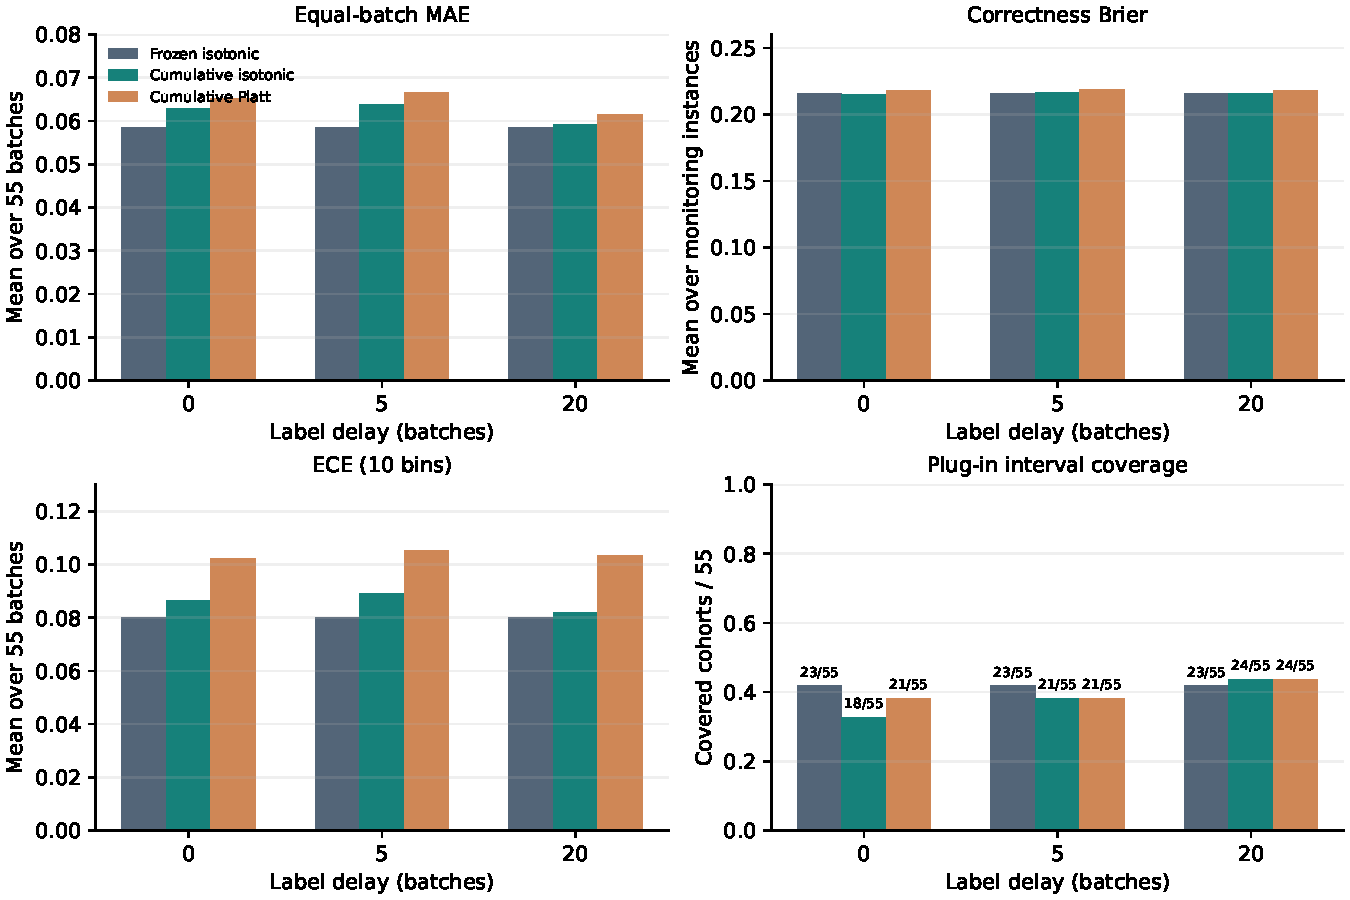
\includegraphics[width=.98\linewidth]{calibration_family.pdf}\caption{Estimation and correctness-calibration metrics by release delay. Lower MAE, Brier and ECE are preferable; coverage counts are shown as fractions out of 55.}
\end{figure}
The frozen calibrator had MAE 0.0586, correctness Brier 0.2160 and ECE$_{10}$ 0.0801 at every delay because its predictions did not change. Cumulative isotonic MAE was 0.0628, 0.0637 and 0.0591 for delays 0, 5 and 20; cumulative Platt MAE was 0.0653, 0.0666 and 0.0615. Both updated methods reduced signed bias toward zero but had worse MAE and ECE than frozen isotonic at every delay. Coverage was mixed (frozen 23/55; updated isotonic 18/55, 21/55, 24/55; Platt 21/55 at all delays). No independent-stream uncertainty interval is estimated.
\section{Interpretation and limitations}
On this one sequence, the lower-bias updates traded off against higher absolute error and poorer ECE. This cautions against treating cumulative recalibration as a fix for external calibration transfer. The single normalized-date ordering has known tied-date ambiguity and is not a second replicate. Serial cohorts are dependent; calibration, reference and interval uncertainty remain omitted. These results do not establish performance on another stream, improved classification, future-harm prediction, or an operational benefit.
\section{Reproduction}
\begin{verbatim}
& C:/Users/hp/anaconda3/python.exe scripts/run_elec2_platt_recalibration.py `
  --run results/phase3/elec2_temporal_20261116_v2 `
  --out results/phase3/elec2_platt_recalibration_NEW
& C:/Users/hp/anaconda3/python.exe scripts/evaluate_elec2_platt_recalibration.py `
  --run results/phase3/elec2_temporal_20261116_v2 `
  --platt results/phase3/elec2_platt_recalibration_NEW `
  --isotonic results/phase3/elec2_recalibration_20261116_v1 `
  --out results/phase3/elec2_calibration_family_NEW
& C:/Users/hp/anaconda3/python.exe scripts/report_elec2_calibration_family.py `
  --run results/phase3/elec2_temporal_20261116_v2 `
  --platt results/phase3/elec2_platt_recalibration_NEW `
  --isotonic results/phase3/elec2_recalibration_20261116_v1 `
  --results results/phase3/elec2_calibration_family_NEW `
  --out reports/phase3/elec2_calibration_family_NEW
\end{verbatim}
\end{document}
